\begin{figure*}[!t]
    \centering
    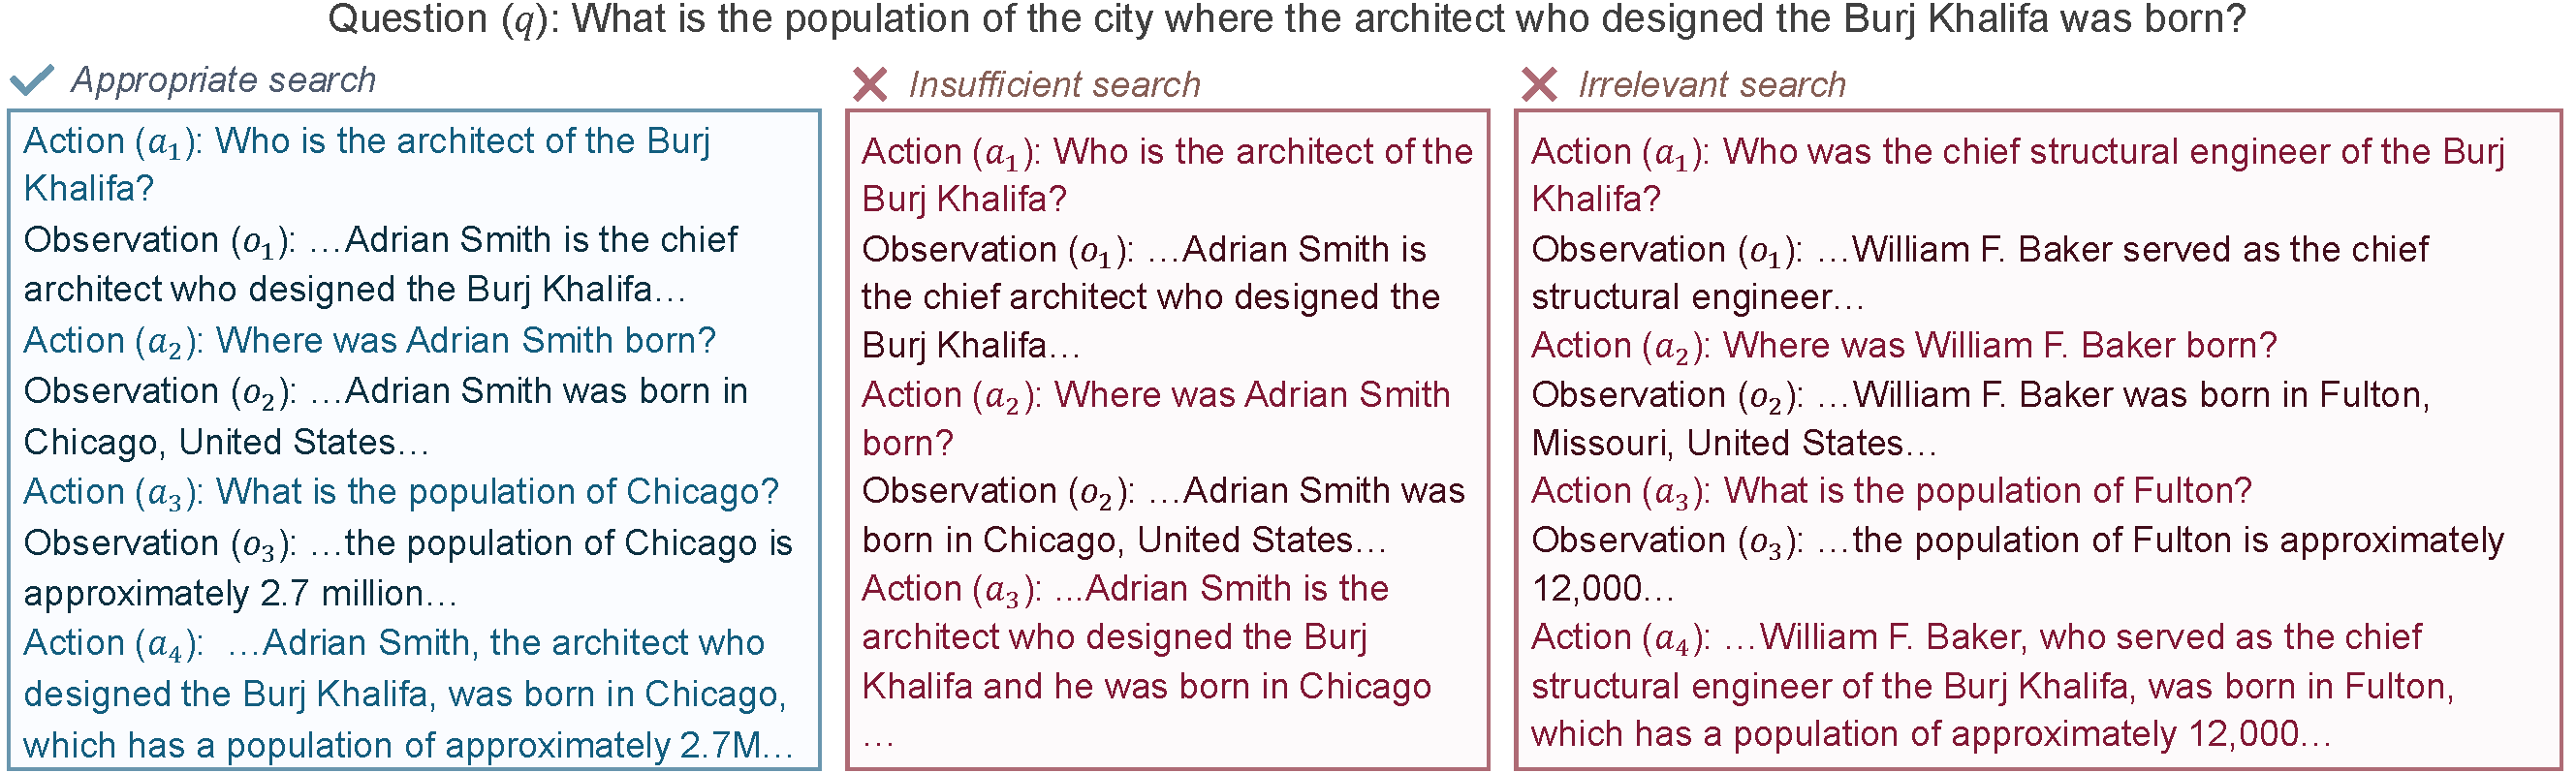
\includegraphics[width=1\linewidth]{img/ccs_ex.pdf}
    \caption{\textbf{Examples of search trajectories.} A high-quality trajectory (left) constitutes a lossless encoding of the question's intent, preserving all necessary information required to reconstruct the original question. In contrast, trajectories that involve insufficient (middle) or irrelevant (right) search steps fail to preserve this information, resulting in incomplete or distorted representations of the question.}
    \label{fig:ccs_ex}
\end{figure*}